\begin{center}
{\huge\textbf{\ttitle}}\\
\end{center}

% =====================================================================
\section{Motivation}

\subsection{Background}
A pressure ulcer is localised damage to skin and underlying tissue, usually over a bony prominence, caused by sustained pressure. Heat and moisture make the skin more vulnerable. Patients who cannot shift their own weight, such as bedridden or post-operative patients, are most at risk, and the sacrum, heels and shoulder blades are the most common sites.

Standard prevention is manual: caregivers reposition the patient roughly every two hours and inspect the skin. This depends on attention and workload, and it gives no objective record of how much pressure, warmth and moisture each region actually experienced between visits.

\subsection{Motivation for this project}
There is a need for a low-cost, continuous and wireless monitor that measures pressure, temperature and humidity at the high-risk body zones, warns caregivers when a zone has been loaded for too long, and can start a corrective action by itself. It must reach caregivers over a distance greater than ordinary Wi-Fi or Bluetooth sensors cover, and it must let them respond remotely.

\subsection{Scope}
The project covers the sensing node, the LoRa transmitter and receiver firmware, the MQTT gateway, and the desktop and mobile dashboards. It is a prototype for demonstration and engineering validation. It is not a certified medical device, and clinical trials, regulatory approval and long-term skin-contact safety testing are outside its scope.

% =====================================================================
\section{Contribution}
The contributions of this project are:
\begin{enumerate}
\item A four-zone sensing node that measures pressure (FSR), temperature and humidity (SHT41 behind an \itwoc{} multiplexer) and runs autonomous therapy and alert logic on the node itself.
\item A compact LoRa uplink packet and a command downlink, so that dashboards can acknowledge alerts and drive motors through the same radio link.
\item An Arduino UNO R4 WiFi gateway that expands the LoRa packet to JSON and bridges it to an MQTT broker, in both directions.
\item A desktop application (Electron) and an Android application (Expo / React Native) with matching features: live charts, compact view, alert lock and acknowledge, CSV export with patient details, and diagnostics.
\item A repeatable simulated test of the whole software chain (broker, simulated telemetry, both dashboards) that does not need the hardware.
\end{enumerate}

\subsection{Organisation of this report}
Section~\ref{sec:lit} reviews the background and the enabling technologies, and Section~\ref{sec:problem} states the problem, objectives and requirements. Section~\ref{sec:method} is the methodology: it explains the development process stage by stage, then the architecture, hardware, firmware, communication design and the two applications. Section~\ref{sec:results} reports testing, results, challenges and limitations, and Section~\ref{sec:summary} gives the conclusion and future work.

% =====================================================================
\clearpage
\section{Literature Survey}
\label{sec:lit}

\subsection{How pressure ulcers develop}
Three physical factors dominate. \emph{Pressure} over a bony prominence compresses small blood vessels and cuts off the tissue's blood supply. A figure of about 32~mmHg, the pressure at which capillaries are commonly reported to close, is widely used as a threshold; it equals 4.27~kPa and is the pressure limit used in this project~\cite{epuap2019}. \emph{Duration} matters as much as magnitude: moderate pressure held for hours causes damage that a short peak does not. \emph{Microclimate}, meaning skin temperature and moisture, changes how quickly tissue breaks down, because warm, damp skin tolerates load and friction poorly.

Because damage builds up over time, the useful signal is not a single reading but how long a zone has stayed above its limit. PressureGuard therefore tracks a continuous ``time above limit'' for each zone and acts after two hours, mirroring the usual repositioning interval.

\subsection{Existing approaches}
{\small\setstretch{1.0}
\begin{table}[H]
\centering
\begin{tabularx}{\textwidth}{@{}>{\raggedright\arraybackslash}p{3.3cm}XX@{}}
\toprule
\textbf{Approach} & \textbf{What it does} & \textbf{Limitation for this problem}\\
\midrule
Scheduled manual repositioning & Caregiver turns the patient about every 2 hours & Depends on staff attention; no objective data per zone\\
Alternating-pressure mattresses & Mattress cells inflate and deflate in cycles & Acts on a fixed cycle, not on measured load; no per-zone record\\
Interface pressure mapping mats & Grid of pressure sensors under the patient & Pressure only; usually wired and used for assessment sessions\\
PressureGuard (this project) & Pressure, temperature and humidity at four zones, local therapy, LoRa link, remote dashboards & Prototype; four zones, one node\\
\bottomrule
\end{tabularx}
\caption{Existing approaches to pressure ulcer prevention compared with PressureGuard.}
\end{table}}

\subsection{Enabling technologies}
{\small\setstretch{1.0}
\begin{table}[H]
\centering
\begin{tabularx}{\textwidth}{@{}>{\raggedright\arraybackslash}p{3.4cm}>{\raggedright\arraybackslash}p{3.6cm}X@{}}
\toprule
\textbf{Technology} & \textbf{Role in the system} & \textbf{Why it was chosen}\\
\midrule
Force-sensitive resistor (FSR) & Pressure at each zone & Thin, low cost, read with a simple voltage divider; needs calibration because its response is non-linear\\
SHT41~\cite{sensirion_sht4x} & Skin-level temperature and humidity & Digital \itwoc{} sensor; every unit has the same address (0x44)\\
TCA9548A~\cite{ti_tca9548a} & \itwoc{} multiplexer (address 0x70) & Lets four identical SHT41 sensors share one bus\\
ESP32 DevKit V1~\cite{espressif_esp32} & Sensor node controller & 12-bit ADC, \itwoc{}, SPI and LEDC PWM on one low-cost board\\
LoRa SX1278 / RA-02, 433~MHz~\cite{semtech_sx1278,loraalliance} & Node-to-gateway radio link & Long range at low power, with small packets that suit periodic readings\\
Arduino UNO R4 WiFi~\cite{arduino_r4} & LoRa receiver and MQTT gateway & Has SPI for the radio and built-in Wi-Fi for the network\\
MQTT~\cite{oasis_mqtt} & Message transport to the dashboards & Lightweight publish/subscribe; many clients can subscribe to the same stream\\
Electron~\cite{electron} & Desktop dashboard & One web-technology code base for Windows and Linux installers\\
Expo / React Native~\cite{expo} & Android dashboard & TypeScript app built into an APK with EAS Build\\
\bottomrule
\end{tabularx}
\caption{Technologies used and the reason for choosing each.}
\end{table}}

\textbf{LoRa in brief.} LoRa is a spread-spectrum modulation that trades data rate for range and sensitivity. Spreading factor and bandwidth set that trade: a higher spreading factor reaches further but takes longer to send a packet. The SX127x family limits a packet to 255 bytes, so the telemetry in this project is sent in a compact format (Section~\ref{sec:packet}).

\textbf{MQTT in brief.} MQTT clients publish messages to named topics on a broker, and any client subscribed to a topic receives them~\cite{oasis_mqtt}. This decouples the gateway from the dashboards: the same telemetry reaches the desktop and the phone without the gateway knowing either exists. A browser or phone cannot open a raw TCP connection, so the phone application uses MQTT over WebSockets~\cite{mqttjs}.

% =====================================================================
\clearpage
\section{Problem Definition and Objective}
\label{sec:problem}

\subsection{Problem statement}
Design and build a low-cost, continuous and wireless monitor that measures pressure, temperature and humidity at the high-risk body zones, warns caregivers when a zone has been loaded for too long, can start a corrective action by itself, and lets caregivers respond remotely.

\subsection{Objectives}
\begin{enumerate}
\item Measure pressure, temperature and humidity at four zones: sacrum, left heel, right heel and shoulder.
\item Detect sustained high load and start therapy motors automatically after two hours, with a local buzzer and LED alert if the condition persists.
\item Transmit compact telemetry over long-range LoRa (433~MHz) and bridge it to Wi-Fi through MQTT.
\item Provide a desktop dashboard and an Android application with live charts, alerts, patient details, CSV export, remote motor control and diagnostics.
\item Allow commands from the dashboards (acknowledge, motor test, diagnostics) to travel back to the sensor node.
\end{enumerate}

\subsection{Functional requirements}
{\small\setstretch{1.0}
\begin{table}[H]
\centering
\begin{tabularx}{\textwidth}{@{}lX@{}}
\toprule
\textbf{ID} & \textbf{Requirement}\\
\midrule
FR1 & Measure pressure, temperature and humidity at four zones (sacrum, left heel, right heel, shoulder) every 5 seconds\\
FR2 & Compare each reading with a per-zone limit: 4.27~kPa pressure (4.00~kPa at the shoulder), 36~\degC{} and 70\,\% relative humidity\\
FR3 & Start the zone's therapy motor for 15 seconds when it has stayed above a limit for 2 hours, then re-check it\\
FR4 & Raise a buzzer and LED alert if the zone is still above a limit after therapy\\
FR5 & Send all zones in one compact packet over LoRa at 433~MHz\\
FR6 & Receive commands from the dashboards (acknowledge alerts, start or stop motors) over LoRa\\
FR7 & Publish telemetry to an MQTT broker and forward dashboard commands to the node\\
FR8 & Show live values and charts for each zone, with a compact view of all four zones\\
FR9 & Flash and lock an alerting zone until a caregiver acknowledges it\\
FR10 & Export a zone's log as a CSV file, with optional patient details\\
FR11 & Provide diagnostics: motor test, FSR calibration and \itwoc{} and sensor scan\\
FR12 & Detect and report loss of telemetry\\
\bottomrule
\end{tabularx}
\caption{Functional requirements.}
\end{table}}

\subsection{Non-functional requirements}
\begin{itemize}
\item \textbf{Range:} the node must not depend on Wi-Fi coverage at the bedside; LoRa provides the radio link.
\item \textbf{Autonomy:} therapy and alert decisions run on the node, so protection continues if the link or a dashboard fails.
\item \textbf{Extensibility:} more than one dashboard must be able to receive the same data without changes to the gateway.
\item \textbf{Consistency:} the desktop and mobile applications use the same topics, payloads and limits.
\item \textbf{Cost and simplicity:} off-the-shelf boards and sensors, with no custom PCB manufacturing required for the prototype.
\end{itemize}

% =====================================================================
\clearpage
\section{Methodology}
\label{sec:method}

\subsection{Development process}
The final system was not built in one step. It grew through five stages, each of which answered a question the previous one raised. This subsection explains how the team approached the project and why the design ended up in its final form.

{\small\setstretch{1.0}
\begin{table}[H]
\centering
\begin{tabularx}{\textwidth}{@{}>{\raggedright\arraybackslash}p{2.3cm}>{\raggedright\arraybackslash}p{4.2cm}>{\raggedright\arraybackslash}p{3.3cm}X@{}}
\toprule
\textbf{Stage} & \textbf{What was built} & \textbf{Main question} & \textbf{Outcome}\\
\midrule
1. Exploration & Test sensors (ECG, sweat, temperature, pulse oximeter) on Raspberry Pi and Arduino; first mobile and desktop dashboards & How do we acquire, transport and display physiological data? & Working acquisition-to-dashboard chain and a starting point for the dashboards\\
2. PressureGuard hardware & Supplied node: ESP32, four FSRs, four SHT41 sensors behind a multiplexer, therapy motors & Does the real hardware read correctly? & Connections corrected and each subsystem verified\\
3. Iterative dashboards & Dashboards for one zone, then four zones, then a diagnostics tab & What does a caregiver need to see and do? & Full-featured desktop and mobile applications\\
4. LoRa split & Firmware split into a LoRa transmitter (node) and receiver (gateway) with MQTT & How do we reach the caregiver over distance and serve many dashboards? & Long-range, broker-based architecture\\
5. Final form & Both dashboards on the MQTT topics, downlink commands, simulated end-to-end testing & Does the complete chain work together? & The system described in this report\\
\bottomrule
\end{tabularx}
\caption{Overview of the five development stages.}
\end{table}}

\subsubsection{Stage 1: Exploration with test sensors}
The team began with a small set of general-purpose sensors rather than the final hardware: an ECG sensor, a sweat sensor, a temperature sensor and a pulse oximeter. They were connected to a Raspberry Pi and to Arduino boards.

The purpose was to learn the whole path a reading takes, not to build the final product. This stage covered how different sensors are interfaced (analog inputs, \itwoc{} and serial), how to sample them at a steady rate, how noisy raw signals look, and how to move values from a microcontroller to a screen.

A first mobile dashboard and a first desktop dashboard were built at this stage. They displayed live values and charts from the test sensors. Building both early proved the idea that one data stream could feed several kinds of client, and it gave the team a working base of live cards, scrolling charts and a patient panel to adapt later.

\subsubsection{Stage 2: The PressureGuard hardware}
The team was then given the actual PressureGuard system: an ESP32 sensing node with four FSRs, four SHT41 sensors reached through a TCA9548A \itwoc{} multiplexer, four therapy motors driven through MOSFETs, a buzzer and LED, and a LoRa module.

The first task was to compare the physical wiring with the schematic and correct the connections that did not match. Each subsystem was then checked on its own before being combined, in this order:
\begin{enumerate}
\item \textbf{FSR channels:} read the raw ADC value and the derived pressure of each zone and confirm that pressing a sensor changes only its own channel.
\item \textbf{\itwoc{} bus:} scan the bus, then open each multiplexer channel in turn and confirm that an SHT41 answers on it.
\item \textbf{Therapy motors:} run each motor in isolation, then all together, to confirm that every motor is wired to its own zone.
\item \textbf{Alert outputs:} confirm the buzzer and the LED.
\end{enumerate}
The firmware of that period offered serial commands for these checks (an \itwoc{} scan, per-zone FSR calibration, and per-zone and all-motor tests). They shaped the diagnostics screen built in Stage 3.

\subsubsection{Stage 3: Dashboards built iteratively}
With the hardware verified, the dashboards were rebuilt around the real data in three increments. In this intermediate architecture the applications read data from the ESP32 directly over Wi-Fi.

\textbf{One zone.} The first version showed a single zone: temperature, humidity and pressure cards, three live charts, and the patient panel. Working with one zone kept the problem small and settled the data format, the refresh behaviour and the chart design before multiplying them by four.

\textbf{Four zones.} The next increment added a tab for each of the four zones and a compact view that shows all four at once. It also added the alert behaviour: an alerting zone's tab flashes, its screen is locked behind an Acknowledge button, and acknowledging sends a command back to the device. Per-zone CSV export was added here.

\textbf{Diagnostics tab.} Finally, the serial checks used in Stage 2 were turned into an in-app diagnostics screen with a motor test, a two-point FSR calibration and an \itwoc{} and sensors scan. This removed the need for a laptop and serial cable to commission a node.

The mobile application followed the same increments and kept feature parity with the desktop application.

\subsubsection{Stage 4: Splitting into a LoRa transmitter and receiver}
In the intermediate design one ESP32 both sensed and served data over Wi-Fi. That limits range to Wi-Fi coverage, ties the node to a particular network, and makes every dashboard a direct client of the node. The team therefore split the firmware in two:
\begin{itemize}
\item \textbf{Transmitter (sensor node):} reads the sensors, applies the thresholds and therapy logic, and sends a compact packet over LoRa. It no longer needs Wi-Fi.
\item \textbf{Receiver (gateway):} receives the LoRa packet, expands it to JSON, and publishes it to an MQTT broker. It also forwards commands from the dashboards back to the node over LoRa.
\end{itemize}
This change had three consequences. The packet had to be made compact enough for a LoRa frame. A downlink path was needed so that Acknowledge and the motor commands still reach the node; this was solved with a short receive window after every uplink. And both dashboards stopped talking to the node and instead subscribed to the broker, so adding a second dashboard cost nothing. The mobile application, which cannot open raw TCP sockets, connects to the broker over WebSockets.

\subsubsection{Stage 5: Final form}
In the final stage the receiver was moved to an Arduino UNO R4 WiFi, the two dashboards were aligned on the same four MQTT topics, and the whole chain was tested end to end with a simulated telemetry source (Section~\ref{sec:results}). The result is the architecture described next.

\subsubsection{Key design decisions and lessons learned}
{\small\setstretch{1.0}
\begin{table}[H]
\centering
\begin{tabularx}{\textwidth}{@{}>{\raggedright\arraybackslash}p{5.2cm}X@{}}
\toprule
\textbf{Decision} & \textbf{Reason}\\
\midrule
Therapy and alert logic runs on the node & The node keeps protecting the patient even if the radio link or the dashboards are down\\
Compact LoRa packet, expanded at the gateway & Fits the 255-byte frame and keeps airtime short; the gateway adds zone names and signal quality (RSSI and SNR)\\
MQTT broker between gateway and dashboards & Any number of dashboards can subscribe without changing the gateway\\
Downlink only in a short window after each uplink & The node only listens briefly after each transmission, which keeps the protocol simple and avoids collisions with its own transmissions\\
Same topics and payloads in desktop and mobile apps & One gateway and one test tool serve both applications\\
\bottomrule
\end{tabularx}
\caption{Key design decisions.}
\end{table}}
Lessons learned: verify each subsystem alone before combining them, because wiring errors are easy to mistake for software faults; build one zone completely before scaling to four; separate the data path (sensing, radio, broker) from the presentation (dashboards) so that either can change independently; and keep diagnostic tools inside the product, since they speed up commissioning and debugging.

\subsection{System architecture}
Figure~\ref{fig:arch} shows the architecture. The system has four parts in a chain, with a reverse path for commands.
\begin{figure}[H]
\centering
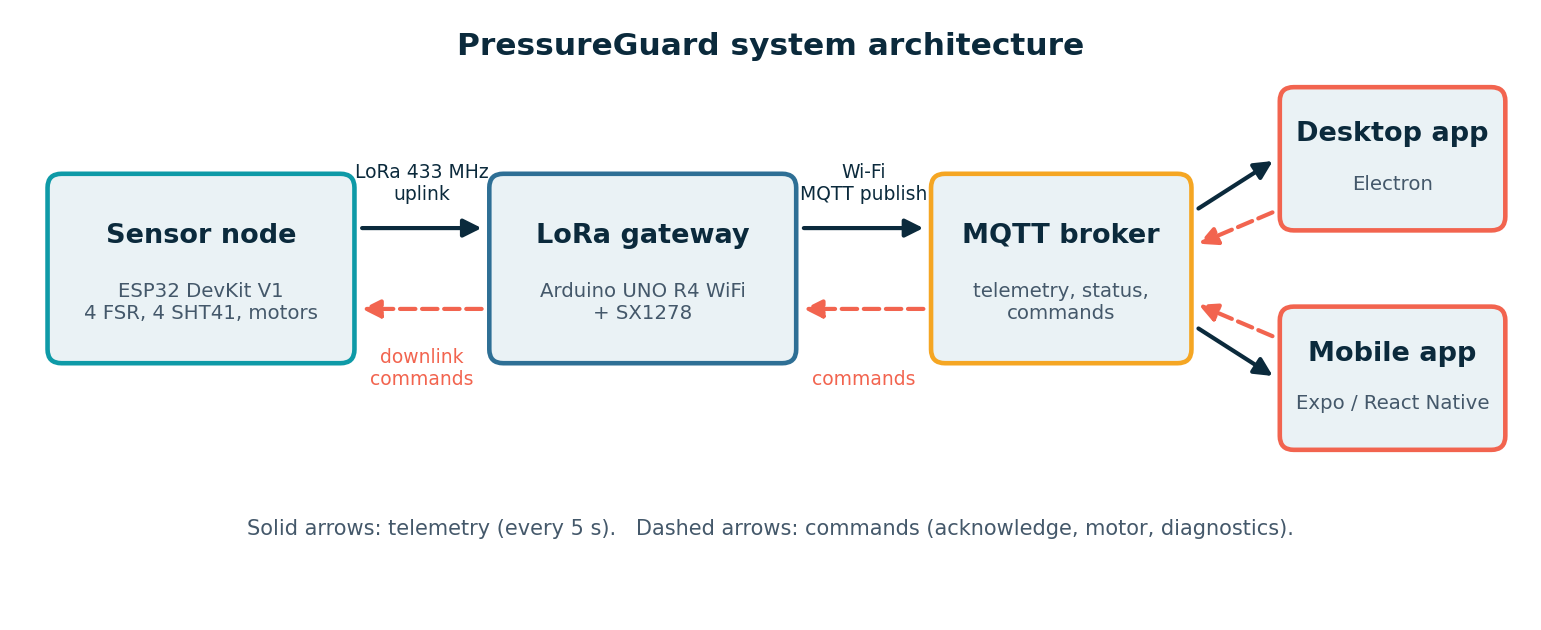
\includegraphics[width=\textwidth]{figs/fig4_1_architecture.png}
\caption{System architecture. Solid arrows carry telemetry; dashed arrows carry commands back to the node.}
\label{fig:arch}
\end{figure}
\begin{enumerate}
\item \textbf{Sensor node (ESP32 DevKit V1).} Reads four FSRs and four SHT41 sensors, runs the threshold, timer, therapy and alert logic, drives the motors, buzzer and LED, and transmits and receives LoRa packets.
\item \textbf{LoRa link (SX1278, 433~MHz).} Carries a compact uplink packet from node to gateway and a short downlink command from gateway to node.
\item \textbf{Gateway (Arduino UNO R4 WiFi with an SX1278).} Receives the LoRa packet, expands it into full JSON, adds the signal quality (RSSI and SNR), and publishes it to the MQTT broker. It subscribes to the command topics and forwards commands to the node.
\item \textbf{MQTT broker and dashboards.} The broker distributes telemetry to the Electron desktop application and the Android application, and carries their commands back.
\end{enumerate}
\textbf{Uplink path.} The node reads sensors every 5~s, then transmits one packet. The gateway receives it, publishes JSON on \tp{pressureguard/telemetry}, and both dashboards update.

\textbf{Downlink path.} A dashboard publishes a command on \tp{pressureguard/commands/ack} or \tp{pressureguard/commands/diag}. The gateway holds it until the next uplink arrives, waits 80~ms, and transmits it. The node listens for 1.5~s after each of its transmissions and executes the command it receives. Because commands ride on the uplink rhythm, a command reaches the node within about one polling interval (up to 5 seconds) of being sent.

\subsection{Hardware design}
\subsubsection{Components}
{\small\setstretch{1.0}
\begin{table}[H]
\centering
\begin{tabularx}{\textwidth}{@{}Xcl@{}}
\toprule
\textbf{Component} & \textbf{Qty} & \textbf{Function}\\
\midrule
ESP32 DevKit V1 & 1 & Sensor node controller\\
Force-sensitive resistor (FSR) & 4 & Pressure at each zone\\
10~\kohm{} resistor (1\,\%) & 4 & Lower leg of each FSR voltage divider\\
SHT41 temperature and humidity sensor & 4 & Skin-level temperature and humidity, \itwoc{} address 0x44\\
TCA9548A \itwoc{} multiplexer & 1 & Gives each SHT41 its own channel (address 0x70)\\
4.7~\kohm{} resistor (1\,\%) & 2 & \itwoc{} pull-ups on SDA and SCL\\
Therapy motor with MOSFET driver & 4 & Per-zone motor, switched by a PWM pin\\
Buzzer and LED & 1 each & Local alert\\
SX1278 / RA-02 LoRa module & 2 & One on the node, one on the gateway (433~MHz)\\
Arduino UNO R4 WiFi & 1 & LoRa receiver and MQTT gateway\\
\bottomrule
\end{tabularx}
\caption{Components of the PressureGuard system.}
\end{table}}

\subsubsection{Sensor node}
Figure~\ref{fig:nodesch} shows the complete node schematic.
\begin{figure}[H]
\centering
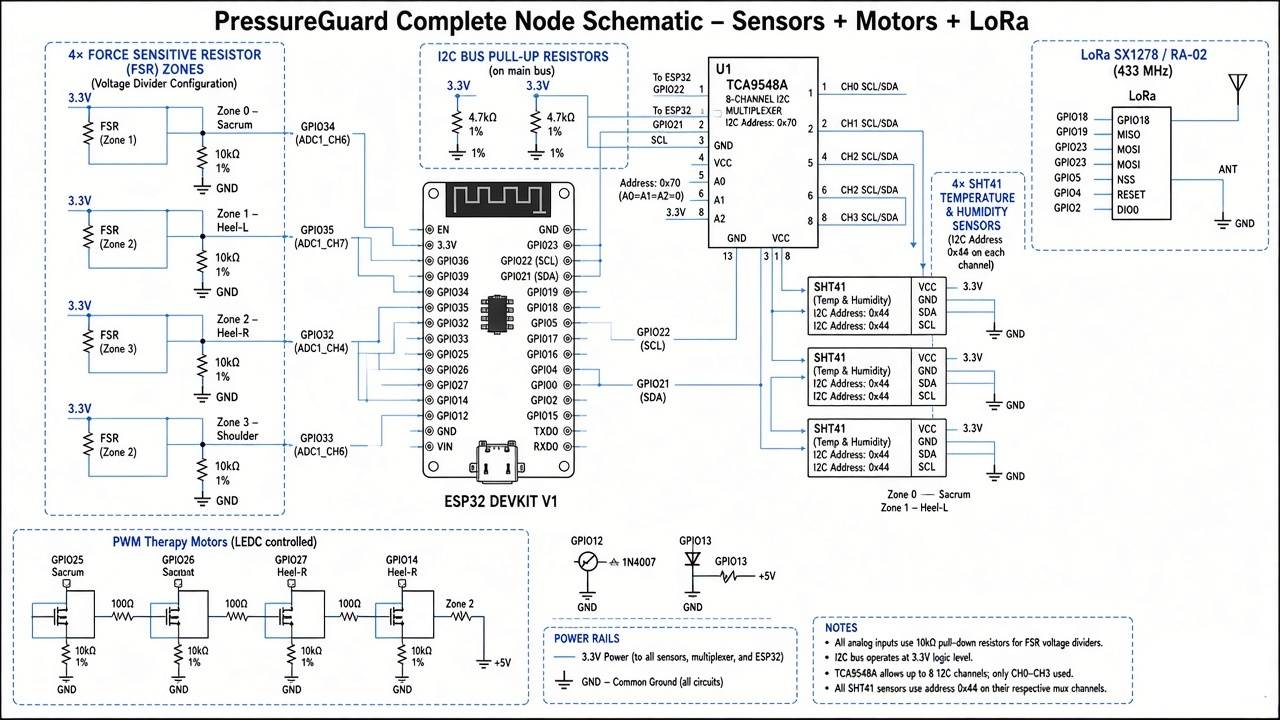
\includegraphics[width=\textwidth]{figs/fig5_1_node_schematic.jpg}
\caption{Complete sensor node schematic: four FSR zones, TCA9548A multiplexer with four SHT41 sensors, therapy motors and the LoRa module.}
\label{fig:nodesch}
\end{figure}

\textbf{Pressure sensing.} Each FSR sits in a voltage divider between 3.3~V and a 10~\kohm{} resistor to ground. The divider midpoint goes to an ADC1 pin of the ESP32. The ADC runs at 12 bits (0 to 4095) with 11~dB attenuation, and each reading is the average of 16 samples taken 200~\textmu s apart to reduce noise. The firmware converts the averaged count to pressure in five steps:
\begin{align}
V &= \frac{\mathrm{raw}\times 3.3}{4095}, &
R_{FSR} &= R_{ref}\,\frac{3.3-V}{V}, &
G &= \frac{1}{R_{FSR}},\\
F &= \frac{G}{k}, &
P &= \frac{F}{A}.
\end{align}
Here $R_{ref}$ is 10~\kohm{}, $k$ is the per-sensor slope constant that relates conductance to force, $A$ is the contact area of the zone, and $P$ is reported in kPa. A count below 15 is treated as no load (0~kPa) and a count above 4080 as saturation (99.9~kPa). The FSR's response is not perfectly linear, which is why the slope $k$ is stored per sensor and can be recalibrated.

{\small\setstretch{1.0}
\begin{table}[H]
\centering
\begin{tabular}{@{}llcc@{}}
\toprule
\textbf{Zone} & \textbf{FSR pin} & \textbf{Contact area (cm\textsuperscript{2})} & \textbf{Pressure limit (kPa)}\\
\midrule
0 Sacrum & GPIO 34 & 90 & 4.27\\
1 Heel-L & GPIO 35 & 45 & 4.27\\
2 Heel-R & GPIO 32 & 45 & 4.27\\
3 Shoulder & GPIO 33 & 60 & 4.00\\
\bottomrule
\end{tabular}
\caption{Zone configuration of the sensor node.}
\end{table}}

\textbf{Temperature and humidity.} Four SHT41 sensors share the same \itwoc{} address, so each is placed on its own channel of the TCA9548A multiplexer. The bus runs at 100~kHz on GPIO~21 (SDA) and GPIO~22 (SCL) with 4.7~\kohm{} pull-ups. To read a zone the firmware opens that channel, sends the high-precision measurement command (0xFD), waits 10~ms, reads six bytes and closes the channel. Temperature is $-45 + 175\times\mathrm{raw}/65535$ in \degC{} and humidity is $-6 + 125\times\mathrm{raw}/65535$ in \% RH, limited to 0--100\,\%.

\textbf{Therapy motors.} Each motor is switched by a MOSFET with a series gate resistor and a pull-down resistor, powered from the 5~V rail. The ESP32 drives the gate with LEDC PWM at 200~Hz, 8-bit resolution and a duty value of 128, which is a 50\,\% duty cycle. The pin is detached and driven low when the motor stops, so the MOSFET gate never floats.

\textbf{Local alert.} A buzzer on GPIO~12 and an LED on GPIO~13 turn on together whenever any zone is in alert.

\subsubsection{LoRa and gateway wiring}
Both radios are SX1278 / RA-02 modules running at 3.3~V logic over SPI. Figure~\ref{fig:gwsch} shows the gateway schematic.
\begin{figure}[H]
\centering
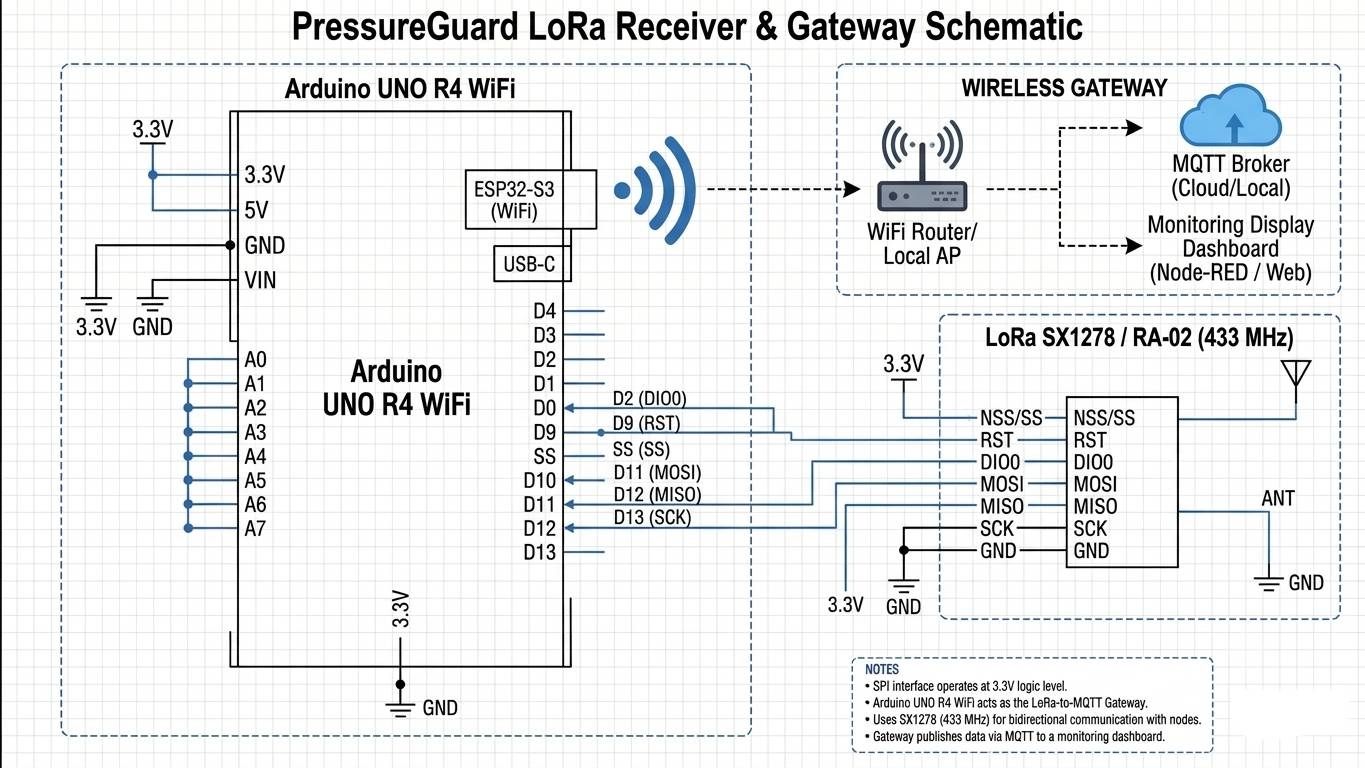
\includegraphics[width=\textwidth]{figs/fig5_2_gateway_schematic.jpg}
\caption{LoRa receiver and gateway schematic: Arduino UNO R4 WiFi, SX1278 module and the Wi-Fi path to the MQTT broker.}
\label{fig:gwsch}
\end{figure}

{\small\setstretch{1.0}
\begin{table}[H]
\centering
\begin{tabular}{@{}lll@{}}
\toprule
\textbf{Signal} & \textbf{ESP32 node} & \textbf{Arduino UNO R4 WiFi gateway}\\
\midrule
SCK & GPIO 18 & D13\\
MISO & GPIO 19 & D12\\
MOSI & GPIO 23 & D11\\
NSS / SS & GPIO 5 & D10\\
RESET & GPIO 4 & D9\\
DIO0 & GPIO 2 & D2\\
\bottomrule
\end{tabular}
\caption{LoRa module connections on the node and on the gateway.}
\end{table}}
The gateway's built-in Wi-Fi connects to the local network, so no separate Wi-Fi module is needed.

\subsubsection{Complete node pin map and power}
{\small\setstretch{1.0}
\begin{table}[H]
\centering
\begin{tabular}{@{}ll@{}}
\toprule
\textbf{Function} & \textbf{Pins}\\
\midrule
FSR zones 0 to 3 & GPIO 34, 35, 32, 33\\
Therapy motors 0 to 3 & GPIO 25, 26, 27, 14\\
Buzzer / LED & GPIO 12 / 13\\
\itwoc{} SDA / SCL & GPIO 21 / 22\\
LoRa SS / RST / DIO0 & GPIO 5 / 4 / 2\\
LoRa SCK / MISO / MOSI & GPIO 18 / 19 / 23\\
\bottomrule
\end{tabular}
\caption{Complete pin map of the sensor node.}
\end{table}}
The ESP32, sensors, multiplexer and LoRa modules run from 3.3~V. The motors run from a 5~V rail, and all grounds are common. The motors draw more current than the logic, so they are switched by MOSFETs rather than directly from the microcontroller pins.

\subsection{Firmware design}
Both programs are written in Arduino C++. They use the LoRa library for the SX1278, ArduinoJson for packet handling, and, on the gateway, WiFiS3 and PubSubClient for Wi-Fi and MQTT.

\subsubsection{Transmitter (sensor node)}
\textbf{Start-up.} The node initialises serial, the \itwoc{} bus (SDA 21, SCL 22, 100~kHz), the 12-bit ADC and all outputs, with every motor pin held low. It then starts the radio at 433~MHz with sync word 0x42, spreading factor 7, 125~kHz bandwidth and 14~dBm. If the radio fails to start, the node stops and reports the error rather than running without a link. It reads all four zones once, sends a first packet and opens a 1.5~s downlink window.

\textbf{Main loop.} Every 5 seconds the node performs the same cycle:
\begin{enumerate}
\item Read each zone: pressure from the FSR, temperature and humidity from the SHT41 on that zone's multiplexer channel.
\item Set the pressure, temperature and humidity ``high'' flags by comparing with the zone's limits.
\item Update the therapy and alert state of each zone (next subsection).
\item Drive the LED and buzzer: on if any zone is in alert, otherwise off.
\item Build and send one compact packet.
\item Wait 50~ms, then listen for a downlink command for 1.5~s and execute it if one arrives.
\end{enumerate}
\textbf{Fault handling.} If an SHT41 does not answer, its temperature and humidity are marked invalid, are sent as zero, and the zone's sensor-OK flag is cleared. An invalid reading never counts as ``high'', so a failed sensor cannot trigger a false alarm. The packet size is checked before sending and must stay within 255 bytes.

\subsubsection{Therapy and alert logic}
Each zone has its own timer and moves through three states.

{\small\setstretch{1.0}
\begin{table}[H]
\centering
\begin{tabularx}{\textwidth}{@{}>{\raggedright\arraybackslash}p{2.3cm}>{\raggedright\arraybackslash}p{4.6cm}X@{}}
\toprule
\textbf{State} & \textbf{Condition} & \textbf{What happens}\\
\midrule
Monitoring & No limit exceeded, or exceeded for less than 2 hours & A timer records when the zone first went high and resets whenever readings return to normal\\
Therapy & Zone has been high continuously for 2 hours & The motor runs at 200~Hz and 50\,\% duty for 15 seconds\\
Alert & After therapy the zone is still high & Buzzer and LED turn on and the alert flag is sent; no further therapy starts while the alert is latched\\
\bottomrule
\end{tabularx}
\caption{Per-zone states of the therapy and alert logic.}
\end{table}}
After the 15 seconds of therapy the node stops the motor and reads the zone again. If any limit is still exceeded the zone enters the alert state; otherwise the timer is cleared and the zone returns to monitoring. An alert is released in two ways: the readings fall back within limits, or a caregiver sends the clear-alerts command. A zone counts as high when its pressure, temperature or humidity is above its limit. The limits are 4.27~kPa (4.00~kPa for the shoulder), 36~\degC{} and 70\,\% RH, and the trigger time is two hours.

\subsubsection{Downlink commands}
The node accepts a small JSON command of at most 256 bytes and acts on its \texttt{action} field.

{\small\setstretch{1.0}
\begin{table}[H]
\centering
\begin{tabularx}{\textwidth}{@{}>{\ttfamily}p{3.2cm}>{\raggedright\arraybackslash}p{3.6cm}X@{}}
\toprule
\textbf{Action} & \textbf{Parameters} & \textbf{Effect on the node}\\
\midrule
motor & \texttt{zone}, \texttt{state} (1 or 0) & Starts a motor and marks the zone as in therapy, or stops it\\
motor\_stop\_all & none & Stops all four motors\\
clear\_alerts & none used & Clears the alert and timer of every zone and switches the LED and buzzer off\\
\bottomrule
\end{tabularx}
\caption{Downlink commands accepted by the node.}
\end{table}}
The \texttt{zone} field sent with \texttt{clear\_alerts} is ignored: the node clears all zones together.

\subsubsection{Receiver (gateway)}
\textbf{Connection.} The gateway joins the Wi-Fi network and then connects to the MQTT broker with a last-will message. It publishes \texttt{online} (retained) on \tp{pressureguard/status} when it connects, and the broker publishes \texttt{offline} on the same topic if the gateway disappears. It subscribes to \tp{pressureguard/commands/#} and enlarges its MQTT buffer to 1800 bytes for the full JSON.

\textbf{Uplink.} When a LoRa packet arrives the gateway parses the compact JSON, adds the radio's RSSI and SNR, and expands each zone row into a named object (Table~\ref{tab:expand}). The result is published on \tp{pressureguard/telemetry}.

{\small\setstretch{1.0}
\begin{table}[H]
\centering
\begin{tabular}{@{}ll@{}}
\toprule
\textbf{Compact field} & \textbf{Expanded field}\\
\midrule
\texttt{s}, \texttt{u} & \texttt{sequence}, \texttt{uptime}\\
row[0] & \texttt{id}, plus \texttt{name} (Sacrum, Heel-L, Heel-R, Shoulder)\\
row[1], row[2], row[3] & \texttt{pressure\_kPa}, \texttt{temperature\_C}, \texttt{humidity\_pct}\\
row[4] bits 0 to 4 & \texttt{pressure\_high}, \texttt{temp\_high}, \texttt{humidity\_high}, \texttt{alert}, \texttt{sensor\_ok}\\
row[5] & \texttt{therapy\_active}\\
\bottomrule
\end{tabular}
\caption{Expansion of the compact packet into named JSON at the gateway.}
\label{tab:expand}
\end{table}}

\textbf{Downlink.} When the gateway receives a command from MQTT it stores it in a single 256-byte slot. After the next uplink has been published it waits 80~ms, so that the node can switch from transmit to receive, and sends the stored command by LoRa. It then clears the slot. Commands are therefore delivered one at a time, in step with the node's 5-second cycle.

\textbf{Why the logic lives on the node.} The therapy timer, alert latch and motor control run entirely on the ESP32. The radio link and the dashboards only observe and override. If the gateway, the broker or an application is offline, the node still starts therapy and raises the local alert on time.

\subsection{Communication design}
\subsubsection{LoRa link parameters}
The node and the gateway use identical radio settings. Matching the sync word keeps unrelated LoRa traffic out.

{\small\setstretch{1.0}
\begin{table}[H]
\centering
\begin{tabular}{@{}ll@{}}
\toprule
\textbf{Parameter} & \textbf{Value}\\
\midrule
Radio & SX1278 / RA-02\\
Frequency & 433~MHz\\
Spreading factor & SF7\\
Bandwidth & 125~kHz\\
Transmit power & 14~dBm\\
Sync word & 0x42\\
Pattern & Uplink every 5~s, then a 1.5~s downlink window\\
\bottomrule
\end{tabular}
\caption{LoRa link parameters.}
\end{table}}
SF7 is the fastest spreading factor, so it keeps each packet short on the air. A higher spreading factor would extend range at the cost of longer packets.

\textbf{Airtime estimate.} For SF7, 125~kHz, coding rate 4/5, an 8-symbol preamble and no CRC, one symbol lasts 1.024~ms. A typical 150-byte packet then takes roughly 0.24~s on the air, and the 255-byte maximum about 0.39~s. Sending every 5 seconds therefore uses about 5\,\% of the time. The 150-byte size is an estimate, not a measured value.

\subsubsection{Uplink packet format}
\label{sec:packet}
To fit four zones into one LoRa frame, the node sends a compact JSON array rather than named fields:
{\small
\begin{verbatim}
{"s":42,"u":3600,"z":[[0,2.35,34.1,56.2,0,0],
 [1,2.08,33.7,57.8,0,0],[2,2.24,34.4,55.2,0,0],
 [3,2.47,33.4,55.1,0,0]]}
\end{verbatim}}
Here \texttt{s} is a sequence number that increases with every packet, \texttt{u} is the node uptime in seconds, and \texttt{z} holds one row per zone: id, pressure (kPa), temperature (\degC), humidity (\% RH), flags and therapy (1 = running). The flags byte packs five conditions (Table~\ref{tab:flags}).

{\small\setstretch{1.0}
\begin{table}[H]
\centering
\begin{tabular}{@{}ccl@{}}
\toprule
\textbf{Bit} & \textbf{Value} & \textbf{Meaning}\\
\midrule
0 & 1 & Pressure above limit\\
1 & 2 & Temperature above limit\\
2 & 4 & Humidity above limit\\
3 & 8 & Alert latched\\
4 & 16 & Sensor readings valid\\
\bottomrule
\end{tabular}
\caption{Meaning of the bits in the flags byte.}
\label{tab:flags}
\end{table}}

\subsubsection{MQTT topics and commands}
The gateway and both dashboards use the same broker (TCP port 1883 for the gateway and desktop application). The mobile application reaches the broker over WebSockets, commonly on port 9001. The gateway subscribes to the wildcard \tp{pressureguard/commands/#}, so any topic under \texttt{commands} reaches the node.

{\small\setstretch{1.0}
\begin{table}[H]
\centering
\begin{tabularx}{\textwidth}{@{}>{\raggedright\arraybackslash}p{4.6cm}>{\raggedright\arraybackslash}p{2.6cm}>{\raggedright\arraybackslash}p{2.2cm}X@{}}
\toprule
\textbf{Topic} & \textbf{Published by} & \textbf{Subscribed by} & \textbf{Content}\\
\midrule
\tp{pressureguard/telemetry} & Gateway & Dashboards & Expanded JSON for all four zones, with RSSI and SNR\\
\tp{pressureguard/status} & Gateway (last will, retained) & Dashboards & \texttt{online} or \texttt{offline}\\
\tp{pressureguard/commands/ack} & Dashboards & Gateway & Acknowledge and alert-clearing commands\\
\tp{pressureguard/commands/diag} & Dashboards & Gateway & Motor test and diagnostic commands\\
\bottomrule
\end{tabularx}
\caption{MQTT topics.}
\end{table}}

{\small\setstretch{1.0}
\begin{table}[H]
\centering
\begin{tabularx}{\textwidth}{@{}>{\raggedright\arraybackslash}p{2.2cm}>{\raggedright\arraybackslash}p{6.2cm}X@{}}
\toprule
\textbf{Command} & \textbf{JSON sent by the dashboard} & \textbf{Result on the node}\\
\midrule
Acknowledge & \texttt{\{"action":"clear\_alerts", "zone":0,"timestamp":...\}} on \texttt{commands/ack} & Clears alerts and timers for all zones\\
Run motor & \texttt{\{"action":"motor","zone":0, "seconds":5,"state":1\}} on \texttt{commands/diag} & Starts the zone's motor; the node stops it after its 15-second therapy period\\
Stop motors & \texttt{\{"action":"motor\_stop\_all"\}} on \texttt{commands/diag} & Stops all motors\\
\bottomrule
\end{tabularx}
\caption{Command messages sent by the dashboards.}
\end{table}}
Diagnostic requests for FSR values, calibration and the \itwoc{} scan are also sent on \texttt{commands/diag}. The current node firmware does not act on them (see Section~\ref{sec:limits}).

\subsubsection{Timing of one cycle}
{\small\setstretch{1.0}
\begin{table}[H]
\centering
\begin{tabularx}{\textwidth}{@{}Xl@{}}
\toprule
\textbf{Step} & \textbf{Time from the start of a cycle}\\
\midrule
Node reads sensors and updates logic & 0~s\\
Node transmits the uplink packet & shortly after 0~s\\
Gateway publishes telemetry to MQTT & within a fraction of a second\\
Gateway sends a queued command (80~ms after publishing) & shortly after the uplink\\
Node listens for the command & 50~ms to 1.55~s after the uplink\\
Next cycle & 5~s\\
\bottomrule
\end{tabularx}
\caption{Timing of one 5-second cycle.}
\end{table}}
Dashboards also watch the age of the last telemetry message and show an offline banner when it stops arriving.

\subsection{Desktop application}
The desktop application gives a caregiver a live view of all four zones on a Windows or Linux computer. It is an Electron application of roughly 2,600 lines of JavaScript, HTML and CSS, packaged into installers with electron-builder~\cite{electron}.

\subsubsection{Structure}
{\small\setstretch{1.0}
\begin{table}[H]
\centering
\begin{tabularx}{\textwidth}{@{}>{\raggedright\arraybackslash}p{5.0cm}X@{}}
\toprule
\textbf{Part} & \textbf{Responsibility}\\
\midrule
Main process (\texttt{main.js}) & Connects to the MQTT broker, subscribes to telemetry and status, publishes commands, and marks the device offline when no telemetry arrives for 15 seconds\\
Preload bridge (\texttt{preload.js}) & Exposes a small, safe set of functions to the interface without giving it direct access to Node.js\\
Interface (\texttt{index.html}, \texttt{renderer.js}) & Draws the tabs, cards, charts, alert screens and patient panel\\
Charts (\texttt{chart-mini.js}) & A small custom charting module for the live graphs\\
Diagnostics (\texttt{diagnostics.js}) & The diagnostics dialog: motor test, FSR calibration and \itwoc{} scan\\
Test tools (\texttt{tools/}) & Mock MQTT and mock device scripts used to exercise the interface without hardware\\
\bottomrule
\end{tabularx}
\caption{Structure of the desktop application.}
\end{table}}
The broker address can be changed in a connection dialog. It can also be set with an environment variable, which is how the simulated tests in Section~\ref{sec:results} pointed the real application at a local broker. The main process, not the interface, owns the MQTT connection. This keeps the connection alive across interface reloads and means the interface never handles sockets directly. Each telemetry message is normalised into one internal shape per zone and then pushed to the interface, so the screen code does not depend on the wire format.

\subsubsection{Features}
{\small\setstretch{1.0}
\begin{table}[H]
\centering
\begin{tabularx}{\textwidth}{@{}>{\raggedright\arraybackslash}p{3.4cm}X@{}}
\toprule
\textbf{Feature} & \textbf{Description}\\
\midrule
Live zone view & One tab per zone (Sacrum, Heel L, Heel R, Shoulder) with cards for temperature, humidity, pressure and status, and three scrolling charts\\
Compact view & All four zones on a single screen with small charts and a status badge each\\
Connection status & A pill in the header shows whether telemetry is arriving; a dialog sets the broker address and saves it for the next launch\\
Alert handling & A red banner lists alerting zones, their tabs flash, and the zone screen is blurred behind a popup that states the cause and an Acknowledge button\\
Acknowledge & Sends the clear-alerts command through MQTT; for 3 seconds afterwards the application ignores a stale alert so the screen does not flicker\\
Recording controls & Play, pause and stop for the charts and the log of each zone\\
Patient details & Name, age, height, weight, diagnosis and bed number for the selected zone\\
CSV export & Saves the zone's timestamped log, with the patient details, to a file\\
Diagnostics & Motor test for each motor or all motors, a two-point FSR calibration with known weights, and an \itwoc{} and sensors scan\\
\bottomrule
\end{tabularx}
\caption{Features of the desktop application.}
\end{table}}

\subsubsection{Screens}
Figures~\ref{fig:d1} to~\ref{fig:d4} show the application running against the simulated telemetry source described in Section~\ref{sec:results}. All values and the patient details are random test data.

\textbf{Live dashboard.} The selected zone's three live values and its status sit above three charts. The patient panel and the Download CSV button are on the left.
\begin{figure}[H]
\centering
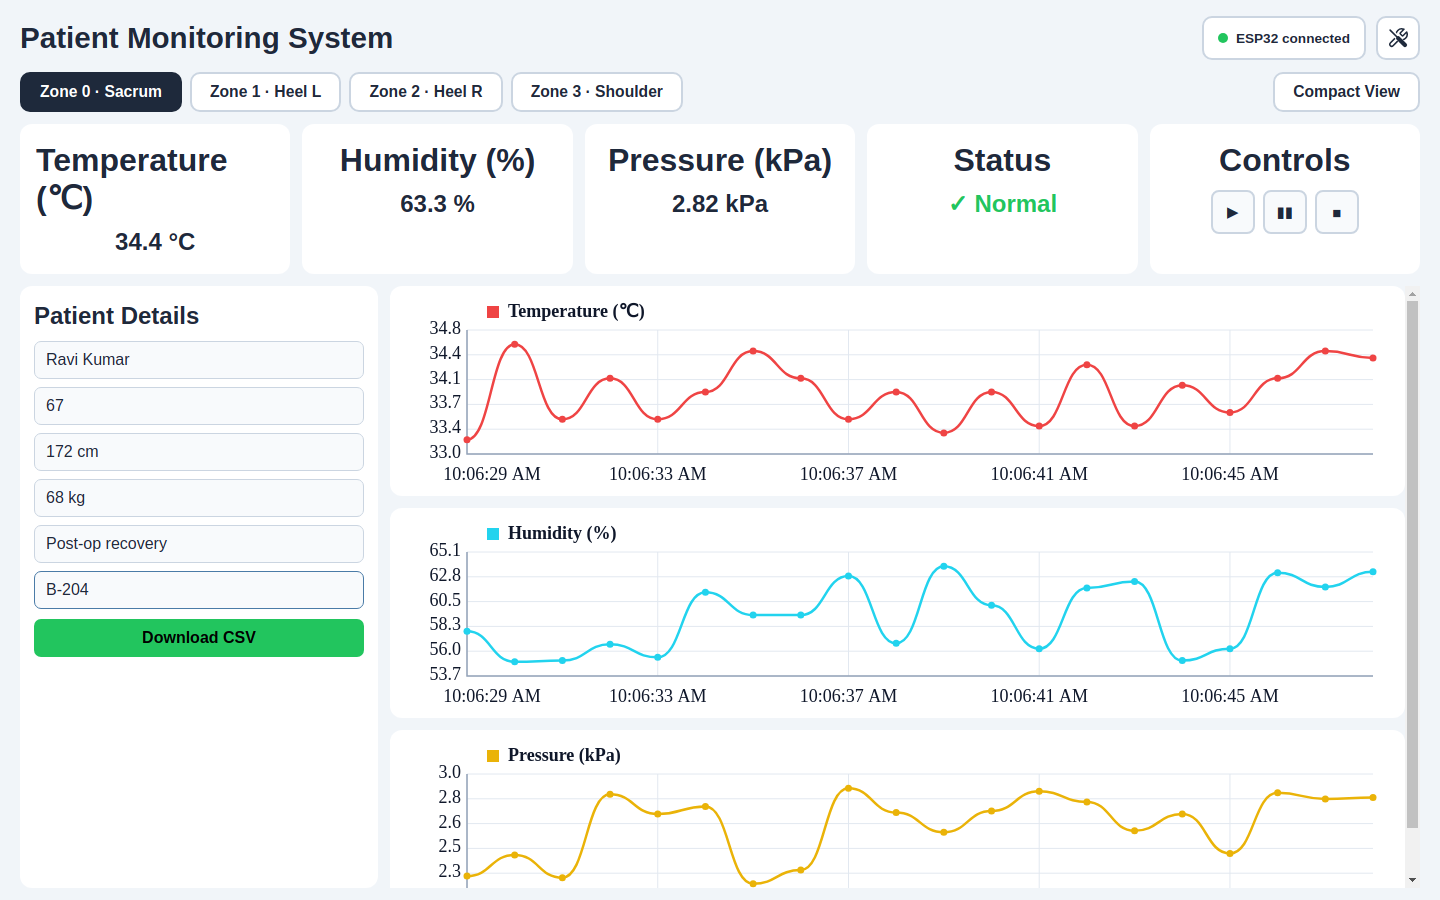
\includegraphics[width=\textwidth]{figs/fig8_1_dashboard.png}
\caption{Live dashboard for Zone 0 (Sacrum) with value cards, charts and the patient panel.}
\label{fig:d1}
\end{figure}

\textbf{Connection dialog.} Accepts an address such as \texttt{mqtt://host:1883}, shows the current connection state and saves the address for the next launch.

\textbf{Compact view.} Four zones at a glance. A zone in alert is blurred and shows its own Acknowledge button, while healthy zones stay readable.
\begin{figure}[H]
\centering
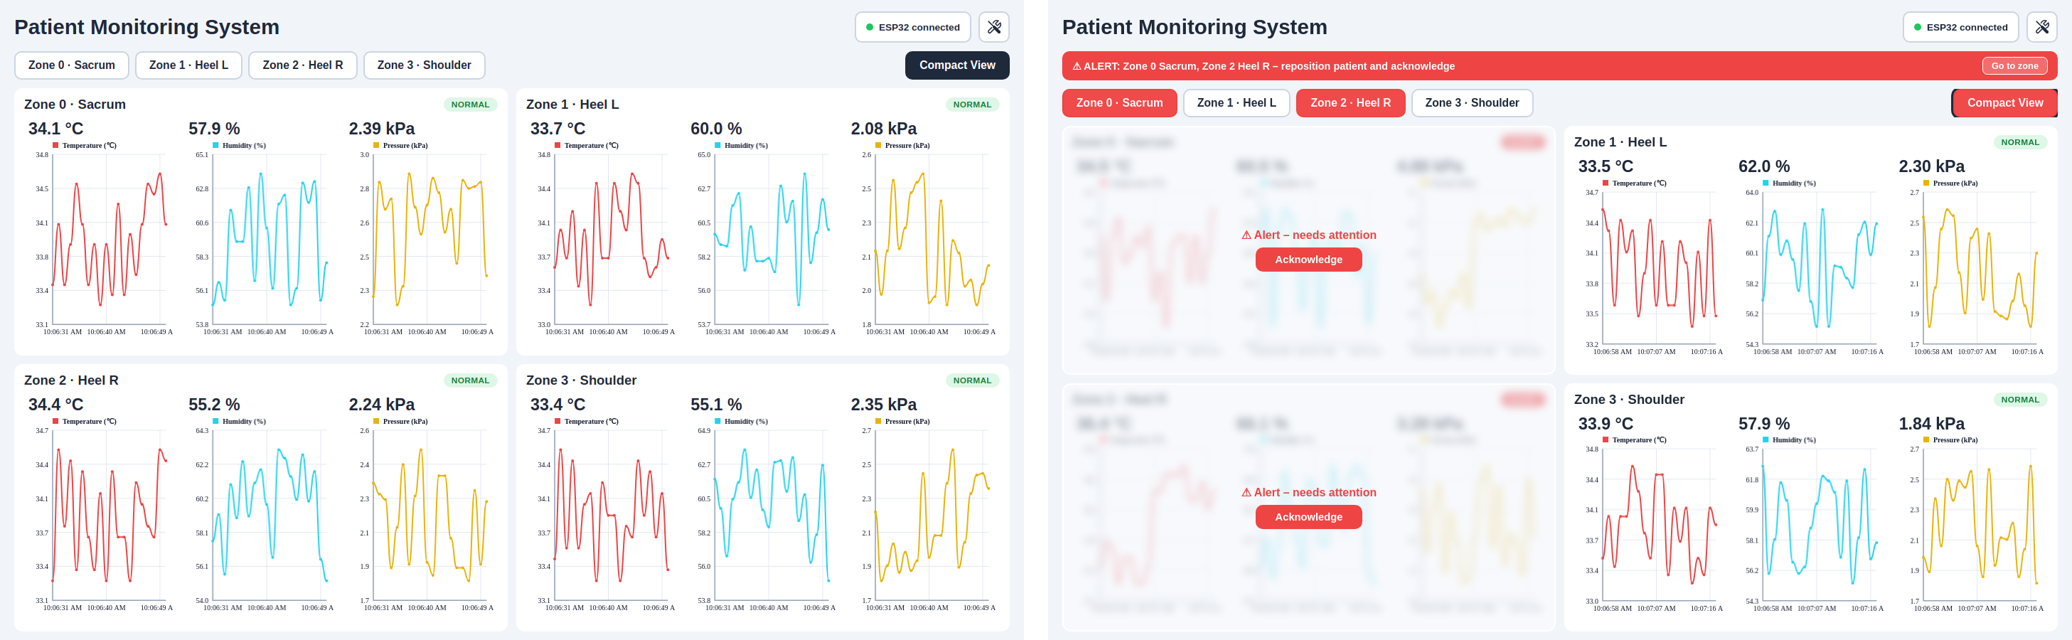
\includegraphics[width=\textwidth]{figs/fig8_2_compact.png}
\caption{Compact view, (a) all zones normal and (b) Sacrum and Heel-R alerting.}
\label{fig:d2}
\end{figure}

\textbf{Alert handling.} The red banner, the flashing tabs and the cause stated in the popup make the alert visible from any tab. The zone stays blurred until a caregiver acknowledges it, and then returns to Normal.
\begin{figure}[H]
\centering
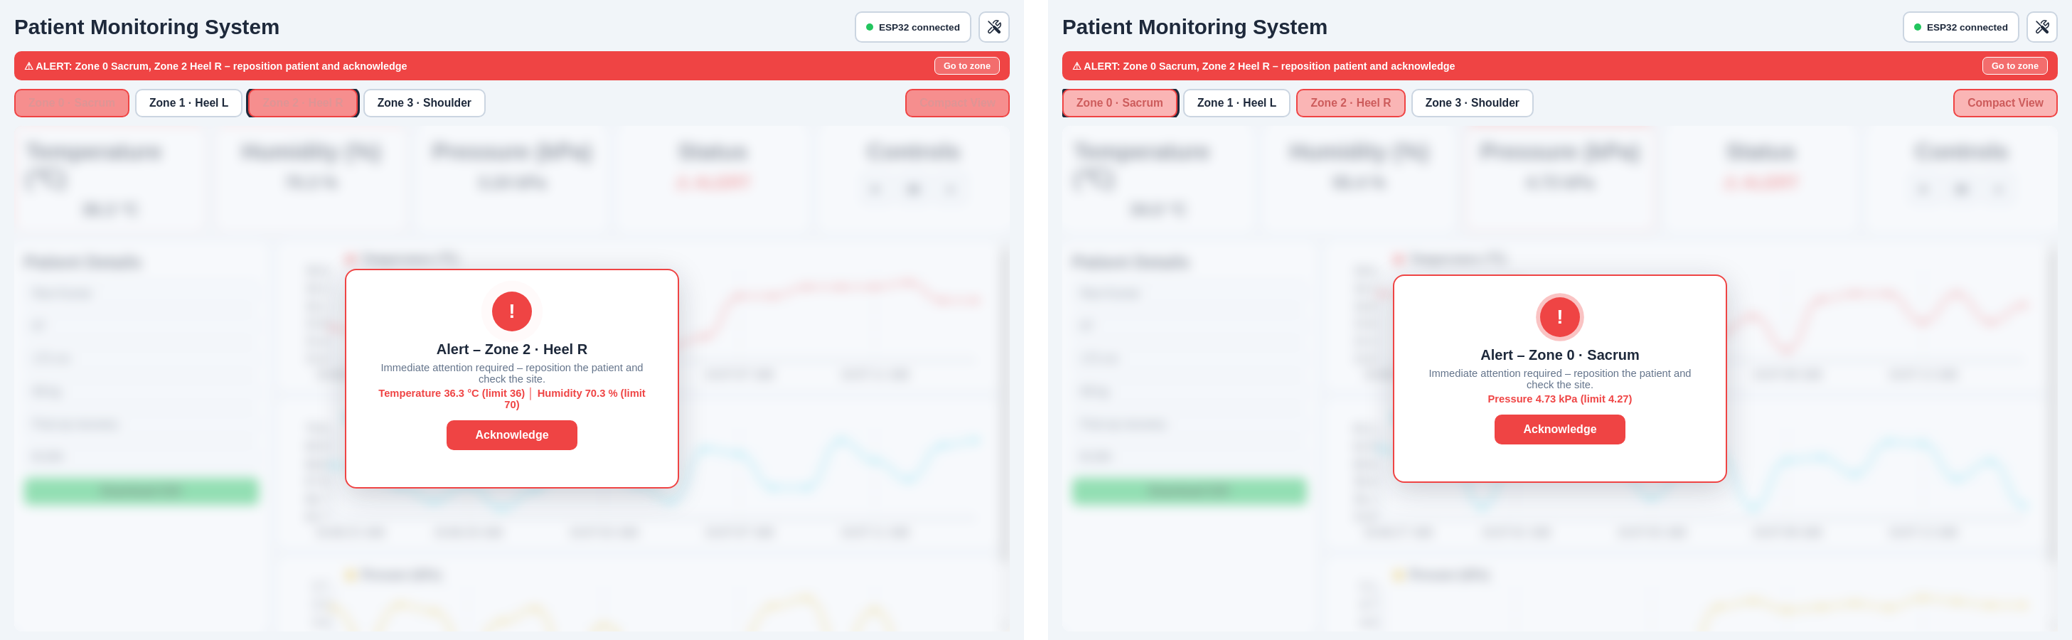
\includegraphics[width=\textwidth]{figs/fig8_3_alert.png}
\caption{(a) Alert raised, with banner, flashing tabs and cause; (b) locked Sacrum zone with the Acknowledge button.}
\label{fig:d3}
\end{figure}

\textbf{Diagnostics.} The dialog offers a motor test and a two-point FSR calibration, together with an \itwoc{} and sensors scan.
\begin{figure}[H]
\centering
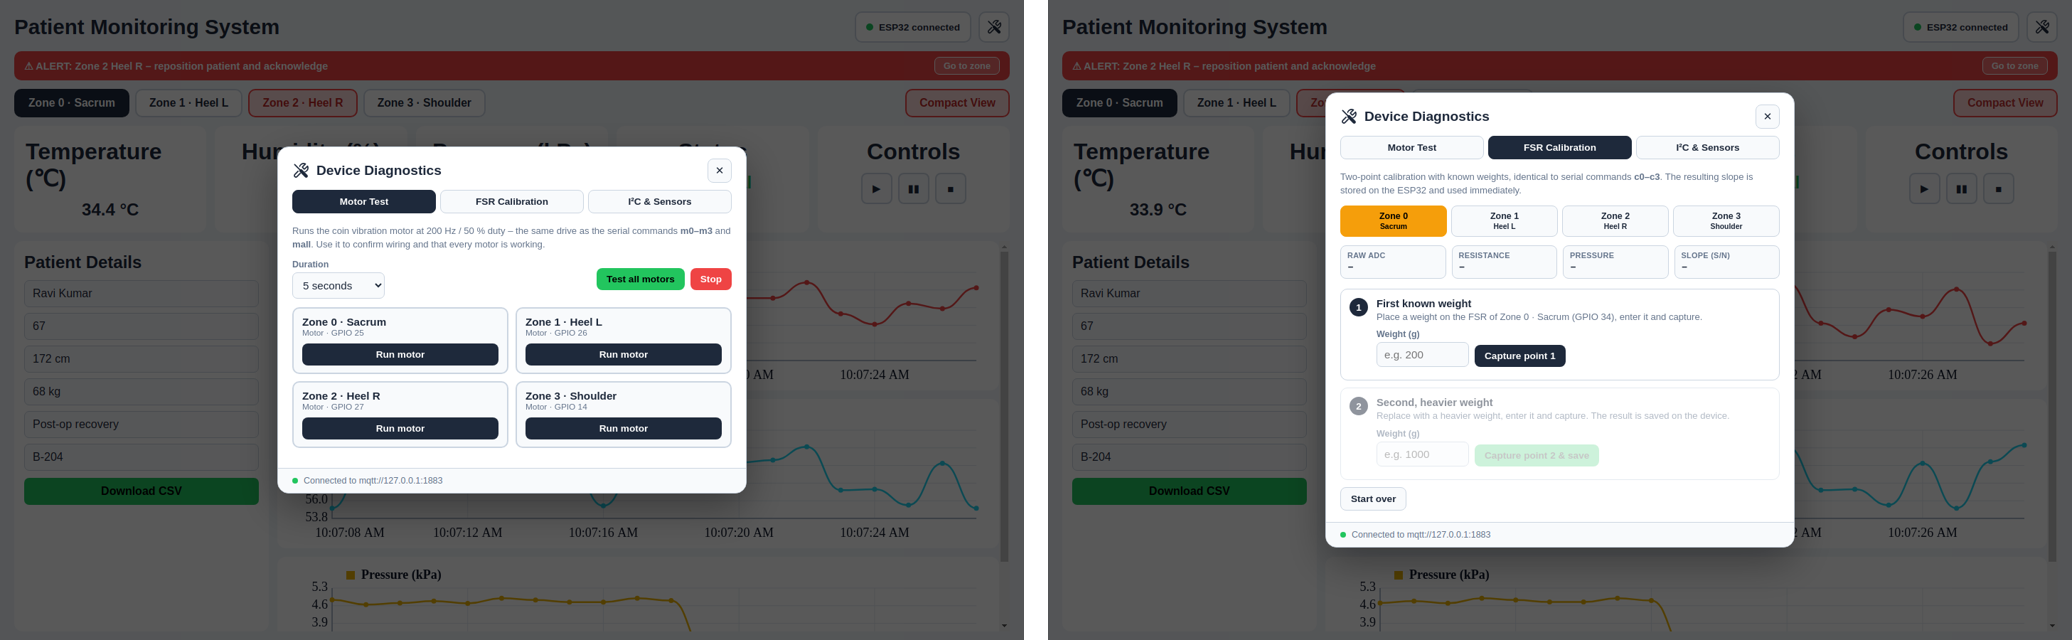
\includegraphics[width=\textwidth]{figs/fig8_4_diag.png}
\caption{Diagnostics dialog, (a) motor test and (b) FSR calibration.}
\label{fig:d4}
\end{figure}

\subsection{Mobile application}
The Android application brings the same monitoring to a caregiver's phone. It is written in TypeScript with Expo and React Native (about 2,000 lines) and built into an installable APK with EAS Build~\cite{expo}. It has the same features and uses the same MQTT topics and payloads as the desktop application.

\subsubsection{Structure}
{\small\setstretch{1.0}
\begin{table}[H]
\centering
\begin{tabularx}{\textwidth}{@{}>{\raggedright\arraybackslash}p{3.2cm}X@{}}
\toprule
\textbf{Part} & \textbf{Responsibility}\\
\midrule
\texttt{api.ts} & MQTT client over WebSockets; a typed \texttt{mqtt://} address is converted to a \texttt{ws://} address automatically; 15-second telemetry timeout\\
\texttt{store.tsx} & Application state: the four zones, history for charts, connection state, alert and acknowledge logic, recording controls\\
\texttt{screens/} & Home, Zone, Settings and Diagnostics screens\\
\texttt{components/} & Zone cards, metrics, charts (drawn with SVG), the alert lock popup, the patient details sheet, badges and icons\\
\texttt{csv.ts} & Builds the CSV text and the file name \texttt{patient\_data\_<Zone>\_<date>\_<time>.csv}\\
\bottomrule
\end{tabularx}
\caption{Structure of the mobile application.}
\end{table}}
A phone cannot open a raw TCP connection to a broker, so the application uses MQTT over WebSockets~\cite{mqttjs}. The broker therefore needs a WebSockets listener, commonly on port 9001. The application checks every 3 seconds that telemetry is still arriving and shows an offline banner after 15 seconds of silence.

\subsubsection{Screens and features}
{\small\setstretch{1.0}
\begin{table}[H]
\centering
\begin{tabularx}{\textwidth}{@{}>{\raggedright\arraybackslash}p{2.7cm}X@{}}
\toprule
\textbf{Screen} & \textbf{What it provides}\\
\midrule
Home & Four zone cards with live temperature, humidity and pressure and a status badge; an alert banner with a View shortcut; a bottom bar showing the connection and opening Diagnostics\\
Zone & Large live values, record, pause and stop controls, three charts with the pressure limit drawn as a dashed line, and Download CSV\\
Alert lock & A frosted, inactive zone with a popup that states the cause and an Acknowledge button\\
Patient sheet & Optional name, age, height, weight, diagnosis and bed number; Save to device (remembers a chosen folder) or Share to another application\\
Settings & Broker address with Save and connect, connection details (gateway IP, signal strength, uptime), and switches for Keep screen on and Alert notifications\\
Diagnostics & Motor test with 3, 5 or 10 second options, FSR two-point calibration, and an \itwoc{} and sensors scan\\
\bottomrule
\end{tabularx}
\caption{Screens and features of the mobile application.}
\end{table}}
Two phone-specific preferences were added. \emph{Keep screen on} stops the phone from sleeping while the application is open, which suits bedside monitoring. \emph{Alert notifications} raise a sound and vibration notification when a zone alerts or telemetry stops.

\subsubsection{Screens in operation}
Figures~\ref{fig:m1} to~\ref{fig:m3} were captured by running the same application code as a web build in a phone-sized window against the simulated telemetry source. They were not captured on a physical phone, so notification sound, vibration and file saving are not shown.

\textbf{Connecting and the home screen.} With the broker unreachable, an orange banner and WAITING badges appear. After the address is saved, the status turns green and shows the gateway details, and the home screen fills with four live cards. Opening a zone shows its values and three charts.
\begin{figure}[H]
\centering
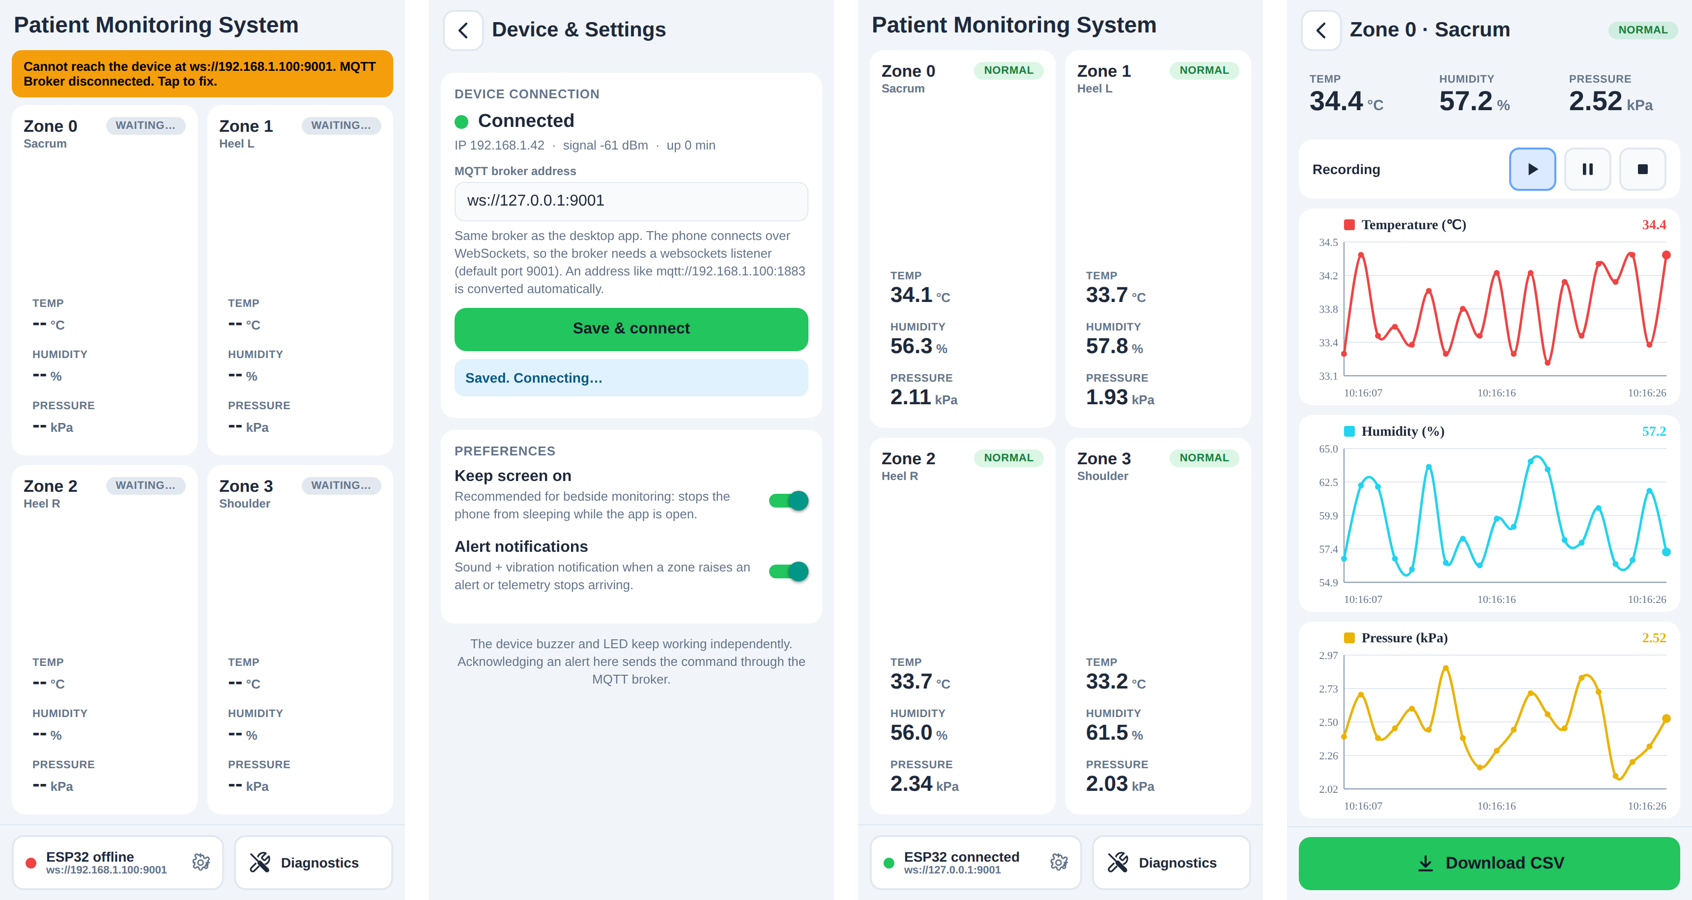
\includegraphics[width=\textwidth]{figs/fig9_1_connect_home.png}
\caption{(a) Offline home screen, (b) settings after connecting, (c) home screen with live zone cards, (d) Zone 0 dashboard.}
\label{fig:m1}
\end{figure}

\textbf{Alert flow.} Alerting cards turn red and a banner lists the zones. Opening a zone shows it locked, with the cause stated and an Acknowledge button. After acknowledging, the zone returns to Normal.
\begin{figure}[H]
\centering
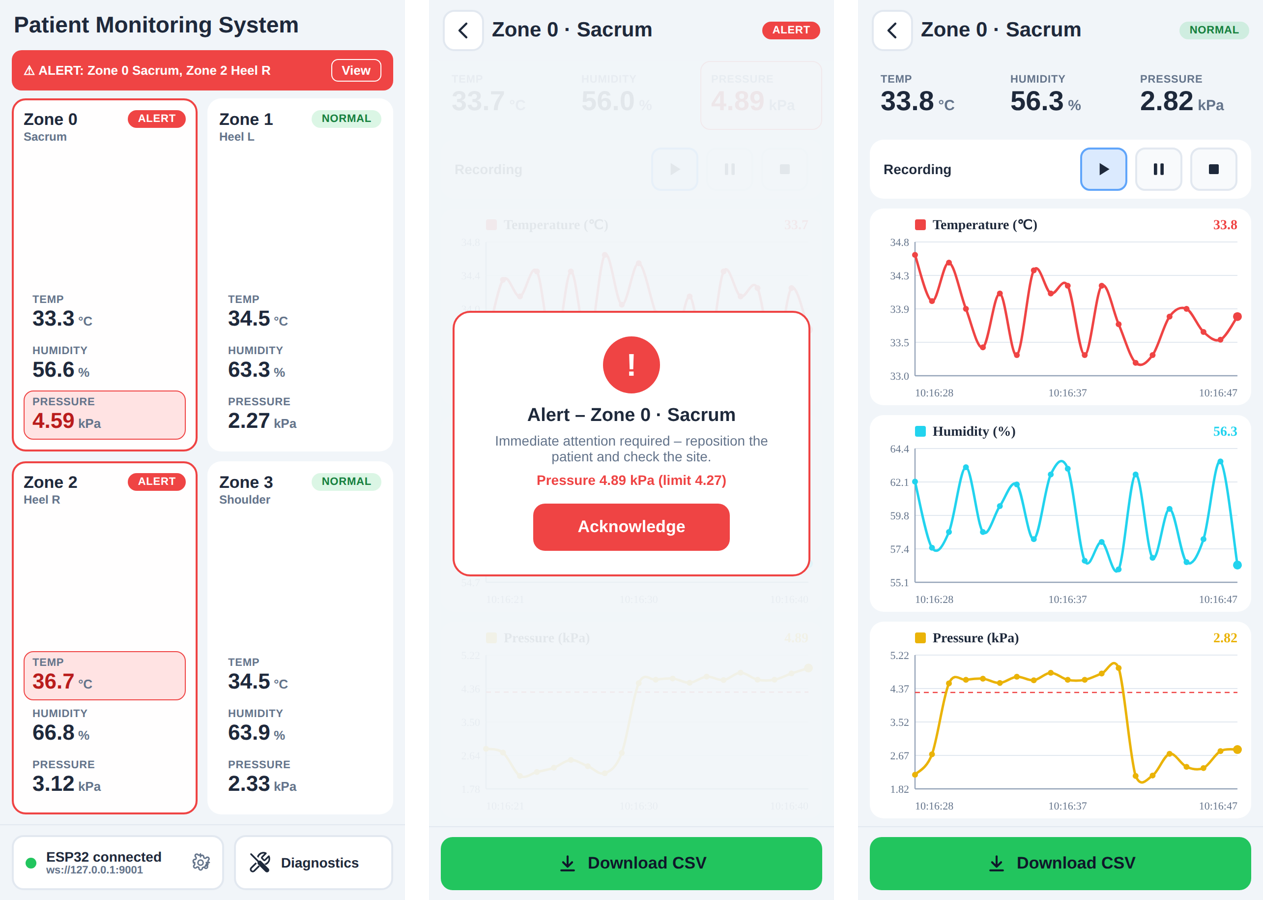
\includegraphics[width=0.8\textwidth]{figs/fig9_2_alert.png}
\caption{(a) Home screen with Sacrum and Heel R alerting, (b) locked Sacrum zone, (c) Sacrum back to Normal after acknowledging.}
\label{fig:m2}
\end{figure}

\textbf{Patient details and diagnostics.} The patient sheet appears before CSV export. The diagnostics screens offer the motor test, FSR calibration and the \itwoc{} scan.
\begin{figure}[H]
\centering
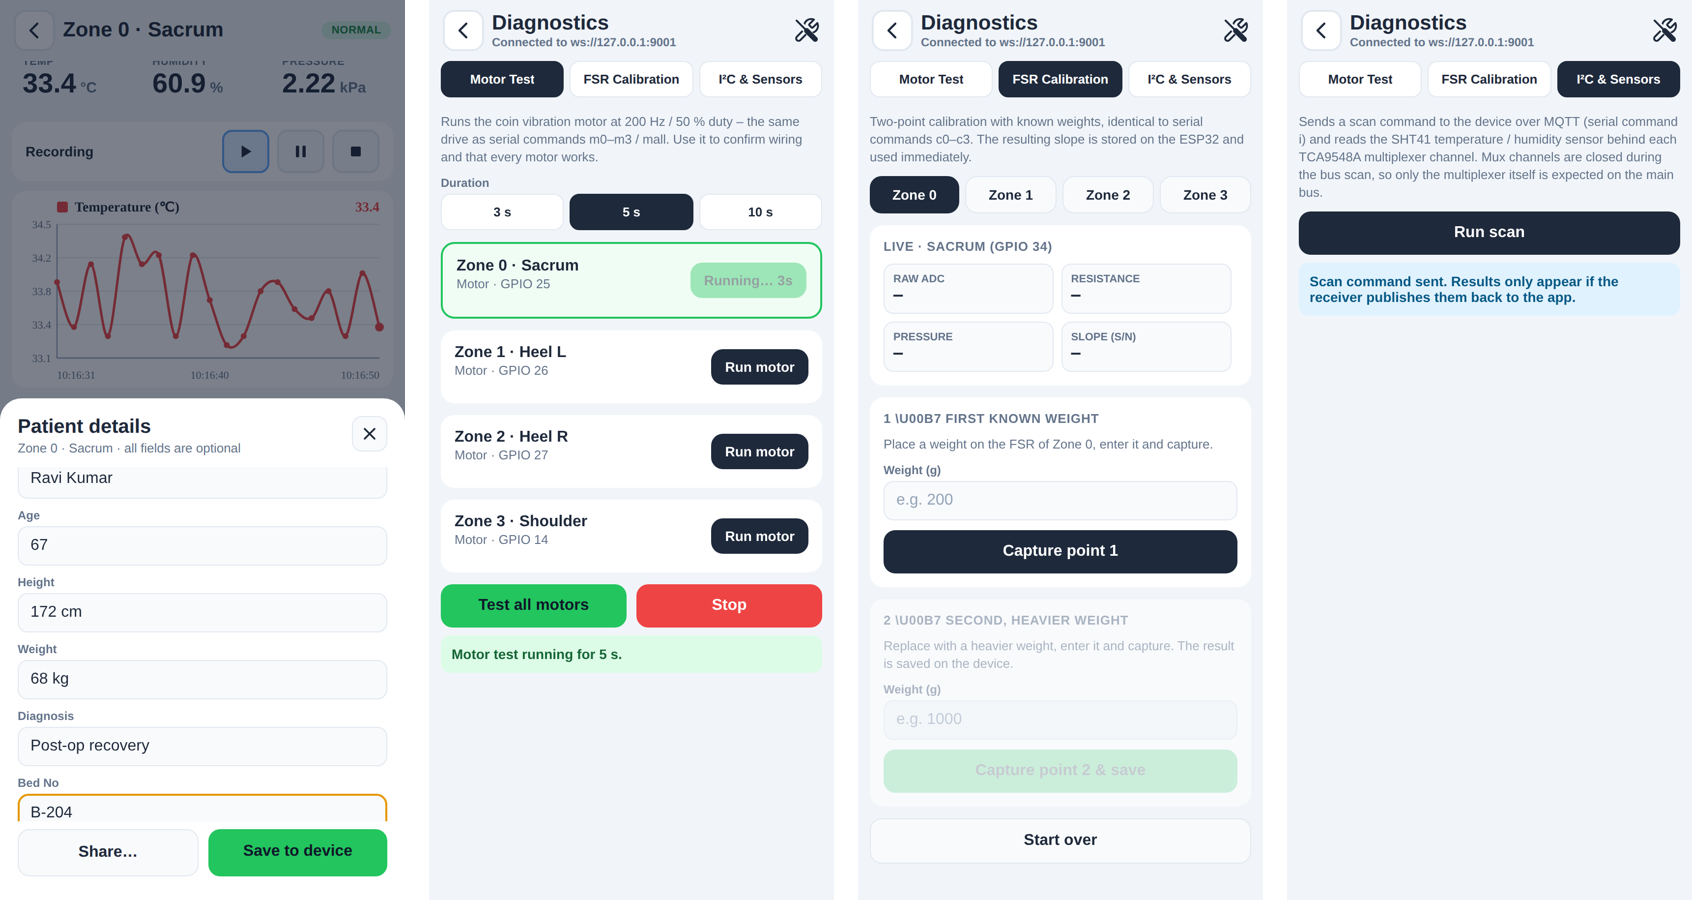
\includegraphics[width=\textwidth]{figs/fig9_3_patient_diag.png}
\caption{(a) Patient details sheet, (b) motor test running, (c) FSR calibration, (d) \itwoc{} and sensors scan.}
\label{fig:m3}
\end{figure}

\subsubsection{Desktop and mobile compared}
{\small\setstretch{1.0}
\begin{table}[H]
\centering
\begin{tabularx}{\textwidth}{@{}>{\raggedright\arraybackslash}p{3.2cm}XX@{}}
\toprule
\textbf{Aspect} & \textbf{Desktop} & \textbf{Mobile}\\
\midrule
Technology & Electron (JavaScript) & Expo / React Native (TypeScript)\\
MQTT transport & TCP, port 1883 & WebSockets, commonly port 9001\\
Views & Zone tabs and compact view & Home cards and zone screen\\
Alert handling & Banner, flashing tabs, lock and acknowledge & Banner, red cards, lock and acknowledge, plus notifications\\
Patient details and CSV & Panel and Download CSV & Bottom sheet, Save to device or Share\\
Diagnostics & Dialog with three tabs & Screen with three tabs\\
\bottomrule
\end{tabularx}
\caption{Comparison of the desktop and mobile applications.}
\end{table}}

% =====================================================================
\clearpage
\section{Results and Analysis}
\label{sec:results}

\subsection{Test approach}
The software chain from gateway output to the two dashboards was tested end to end with a simulated telemetry source. A local MQTT broker was started together with a script that publishes four-zone telemetry once per second in the JSON shape the applications use internally (both applications also accept the gateway's longer field names, such as \texttt{pressure\_kPa}). The real desktop application was run against it, and the mobile application code was run as a web build in a phone-sized window. The script moves through three phases: normal readings, rising pressure, and alerts on the Sacrum (pressure above 4.27~kPa) and Heel-R (temperature above 36~\degC{} and humidity above 70\,\%). It also listens for commands and clears its alerts when it receives an acknowledgement. All readings and the patient shown (a fictional name, age and bed number) are random test data.

This tests the dashboards, the MQTT topics and the command path. It does not test the sensors, the radio or the node firmware, which are covered in Section~\ref{sec:notcovered}.

\subsection{Test cases}
{\small\setstretch{1.0}
\begin{table}[H]
\centering
\begin{tabularx}{\textwidth}{@{}>{\raggedright\arraybackslash}p{0.9cm}>{\raggedright\arraybackslash}p{3.6cm}>{\raggedright\arraybackslash}p{4.0cm}X@{}}
\toprule
\textbf{ID} & \textbf{Test} & \textbf{Expected result} & \textbf{Observed}\\
\midrule
T1 & Open the mobile application with the broker unreachable & Offline banner and WAITING badges & As expected\\
T2 & Enter the broker address and connect (both applications) & Status turns to connected; telemetry starts to flow & As expected; the mobile settings screen shows gateway details\\
T3 & Watch live charts on the zone screens & Values and charts update every second & As expected on both applications\\
T4 & Open the desktop compact view & Four zones with values, charts and a NORMAL badge each & As expected\\
T5 & Raise alerts from the simulator & Banner, flashing tabs, locked zone and a popup naming the cause & As expected: e.g.\ ``Pressure 4.73 kPa (limit 4.27)'' on the desktop and ``Pressure 4.89 kPa (limit 4.27)'' on the phone\\
T6 & Acknowledge the alert & Clear-alerts command published on \texttt{commands/ack}; zone returns to Normal & As expected on both applications; the broker received the \texttt{clear\_alerts} message\\
T7 & Start a motor from the mobile diagnostics screen & Motor command published on \texttt{commands/diag}; row shows a countdown & As expected; broker received the \texttt{motor} message for zone 0, 5 seconds\\
T8 & Request an FSR reading and an \itwoc{} scan & Diagnostic commands published; results appear only if the receiver publishes them back & Commands published; no results returned, because the simulator does not implement them\\
T9 & Open the patient details sheet before CSV export & Optional fields accept input & As expected; saving to a file was not part of this test\\
T10 & Compare compact view in normal and alert states & Alerting zones blurred with their own Acknowledge button; healthy zones readable & As expected on the desktop\\
\bottomrule
\end{tabularx}
\caption{Test cases for the simulated end-to-end test.}
\end{table}}

\subsection{Results}
In the simulated tests the desktop and mobile applications connected to the broker, displayed live telemetry, detected and presented alerts with the correct cause, and published the acknowledge and motor commands on the intended topics. The 3-second post-acknowledge grace period prevented a stale alert from reappearing on screen. The topic names used by the dashboards agree with the gateway design for telemetry and commands. The gateway's own output was not part of this test; its field names are handled by the applications' parsing code, which accepts both naming styles.

\subsection{What the simulation does not cover}
\label{sec:notcovered}
The following need measurements on the real hardware and are not claimed by these tests:
\begin{itemize}
\item LoRa range, packet loss and signal quality (RSSI and SNR) in the intended environment.
\item Accuracy of the pressure reading after FSR calibration against known weights.
\item Therapy timing on the real node, including the two-hour trigger. For a bench test the trigger time can be shortened in the firmware constant.
\item Motor behaviour and power draw under load.
\item Behaviour of the notification sound and vibration, and saving of CSV files, on a physical Android phone.
\end{itemize}

\subsection{Challenges met and how they were handled}
{\small\setstretch{1.0}
\begin{table}[H]
\centering
\begin{tabularx}{\textwidth}{@{}>{\raggedright\arraybackslash}p{5.4cm}X@{}}
\toprule
\textbf{Challenge} & \textbf{How it was handled}\\
\midrule
Some connections on the supplied hardware needed correcting & Wiring was corrected, then each subsystem (FSRs, \itwoc{} bus, motors, alert outputs) was verified on its own before integration\\
Four SHT41 sensors share one \itwoc{} address & A TCA9548A multiplexer gives each sensor its own channel\\
FSR output is non-linear and varies between sensors & Per-sensor slope constant with a two-point calibration procedure in the diagnostics screens\\
LoRa frames are limited to 255 bytes & Compact array packet on the air, expanded to named JSON at the gateway\\
A radio cannot send and receive at once & The node listens for commands in a 1.5~s window after each transmission; the gateway waits 80~ms before replying\\
Phones cannot open raw MQTT connections & The mobile application uses MQTT over WebSockets\\
A stale alert reappeared immediately after acknowledging & A 3-second grace period in both applications\\
Keeping two dashboards consistent & Same topics, payloads and limits, and one shared set of mock and simulation tools\\
\bottomrule
\end{tabularx}
\caption{Challenges and how they were handled.}
\end{table}}

\subsection{Limitations}
\label{sec:limits}
\begin{enumerate}
\item \textbf{Calibration.} The FSR slope is a default value, and an FSR is better suited to detecting load changes than to absolute pressure. Each sensor needs calibration against known weights, and mounting affects the reading.
\item \textbf{One node and one gateway.} The design covers a single patient with four zones. More beds would need node addressing in the packet.
\item \textbf{No security layer.} LoRa packets and MQTT messages are not encrypted or authenticated, and network settings are constants in the firmware.
\item \textbf{Fixed clinical settings.} Limits and the two-hour trigger are set in the node firmware and cannot yet be changed from the dashboards.
\item \textbf{Diagnostic read-back not implemented.} The dashboards send FSR, calibration and \itwoc{} scan requests, but the node firmware does not act on them yet, so those screens receive no results. The motor test also runs for the fixed 15-second therapy period whatever duration is chosen.
\item \textbf{Acknowledge is global.} The clear-alerts command resets every zone, although the dashboards send a zone number with it.
\item \textbf{Command latency.} A command is delivered in step with the node's cycle, so it can take up to about 5 seconds, and the gateway keeps only one pending command.
\item \textbf{Status topic names.} The gateway publishes its online or offline state on \tp{pressureguard/status}, while both dashboards subscribe to \tp{pressureguard/receiver/status}. One side needs to be changed so that the dashboards can show the gateway state.
\item \textbf{Regulatory.} Permitted frequency, power and duty cycle for 433~MHz differ between countries and must be checked before any deployment.
\item \textbf{Medical status.} The system is an engineering prototype. It has not been clinically validated and is not a certified medical device.
\item \textbf{Test coverage.} The dashboards were tested with simulated telemetry only; hardware measurements are listed in Section~\ref{sec:notcovered}.
\end{enumerate}

% =====================================================================
\clearpage
\section{Summary and Future plan of work}
\label{sec:summary}

\subsection{Summary}
PressureGuard demonstrates that the three conditions behind pressure ulcers (sustained pressure, heat and moisture) can be watched continuously at the highest-risk body zones, and that a simple, autonomous response can follow. The sensor node measures four zones every five seconds, compares them with per-zone limits and, after two hours above a limit, runs a therapy motor and raises a local alert if the condition persists. Because this logic runs on the node, protection does not depend on the network.

A LoRa link carries compact telemetry to an Arduino UNO R4 WiFi gateway, which publishes to MQTT so that a desktop application and an Android application can show the same live data, alert caregivers, export logs, and send acknowledge, motor and diagnostic commands back to the node.

The project followed a deliberate path: general-purpose sensors on a Raspberry Pi and Arduino to learn the data chain; correction and verification of the supplied PressureGuard hardware; dashboards grown from one zone to four zones and a diagnostics tab; and finally a split of the firmware into a LoRa transmitter and receiver. The software chain was verified end to end with simulated telemetry. The main outcomes are:
\begin{itemize}
\item A working four-zone sensing and therapy node with local alerts.
\item A two-way LoRa to MQTT gateway design.
\item A desktop application and an Android application with matching features.
\item A documented command and telemetry interface that further clients can reuse.
\end{itemize}

\subsection{Future plan of work}
{\small\setstretch{1.0}
\begin{table}[H]
\centering
\begin{tabularx}{\textwidth}{@{}>{\raggedright\arraybackslash}p{3.0cm}X@{}}
\toprule
\textbf{Area} & \textbf{Improvement}\\
\midrule
Measurement & Per-sensor calibration stored on the node, and a slimmer sensor layout such as a mat or patch\\
Diagnostics & Implement the node side of the FSR, calibration and \itwoc{} scan requests so the diagnostics screens show results\\
Commands & Per-zone acknowledge, and remote change of limits and trigger time\\
Scale & Node addressing and LoRaWAN for many beds on one gateway\\
Security & Encrypted LoRa payloads, MQTT authentication and TLS\\
Intelligence & Risk prediction from pressure, temperature and humidity history, and repositioning reminders\\
Power & Battery operation with low-power sleep between cycles\\
Connectivity & Cloud dashboards and integration with hospital record systems\\
Validation & Range tests, calibration accuracy tests and a supervised clinical evaluation\\
\bottomrule
\end{tabularx}
\caption{Future plan of work.}
\end{table}}




\section*{Appendix}
\addcontentsline{toc}{section}{Appendix}

\subsection*{Appendix A: Source files}
{\small\setstretch{1.0}
\begin{table}[H]
\centering
\begin{tabularx}{\textwidth}{@{}>{\raggedright\arraybackslash}p{3.2cm}>{\raggedright\arraybackslash}p{5.3cm}X@{}}
\toprule
\textbf{Component} & \textbf{File or folder} & \textbf{Description}\\
\midrule
Sensor node firmware & \texttt{final\_transmitter.ino} & ESP32 sensing, therapy and alert logic, LoRa uplink and downlink\\
Gateway firmware & \texttt{final\_receiver.ino} & LoRa receive, JSON expansion, MQTT publish and command forwarding\\
Desktop application & \texttt{main.js}, \texttt{preload.js}, \texttt{renderer.js}, \texttt{index.html}, \texttt{chart-mini.js}, \texttt{diagnostics.js} & Electron application\\
Desktop test tools & \texttt{tools/mock-mqtt.js}, \texttt{tools/mock-esp32.js} & Mock sources for testing without hardware\\
Mobile application & \texttt{src/api.ts}, \texttt{src/store.tsx}, \texttt{src/screens/}, \texttt{src/components/}, \texttt{src/csv.ts} & Expo / React Native application\\
\bottomrule
\end{tabularx}
\end{table}}

\subsection*{Appendix B: Key firmware constants}
{\small\setstretch{1.0}
\begin{table}[H]
\centering
\begin{tabular}{@{}ll@{}}
\toprule
\textbf{Constant} & \textbf{Value}\\
\midrule
Polling interval & 5 seconds\\
Downlink listening window & 1.5 seconds, starting 50~ms after the uplink\\
Therapy trigger & 2 hours continuously above a limit\\
Therapy duration & 15 seconds\\
Motor PWM & 200~Hz, 8-bit, duty 128 (50\,\%)\\
ADC & 12-bit, 11~dB attenuation, 16 samples averaged\\
Pressure limits & 4.27~kPa (sacrum, heels), 4.00~kPa (shoulder)\\
Temperature limit & 36~\degC\\
Humidity limit & 70\,\% RH\\
LoRa & 433~MHz, SF7, 125~kHz, 14~dBm, sync word 0x42\\
Maximum LoRa packet & 255 bytes\\
Gateway downlink delay & 80~ms after publishing\\
Dashboard offline timeout & 15 seconds\\
Acknowledge grace period & 3 seconds\\
\bottomrule
\end{tabular}
\end{table}}

\subsection*{Appendix C: Reproducing the simulated test}
\begin{enumerate}
\item Start an MQTT broker that listens on TCP port 1883 and, for the mobile application, WebSockets on port 9001.
\item Run a script that publishes four-zone telemetry once per second on \tp{pressureguard/telemetry}, moving from normal readings to rising pressure to alerts, and that listens on \tp{pressureguard/commands/#}.
\item Start the desktop application with the environment variable \texttt{MQTT\_BROKER\_URL} set to the broker, or enter the address in its connection dialog.
\item For the mobile application, enter a \texttt{ws://} address in the Settings screen and tap Save and connect.
\item Raise alerts from the script, acknowledge them in the application, and check that the command appears on \tp{pressureguard/commands/ack}.

\end{enumerate}
